\usetikzlibrary{shapes, arrows}
\usetikzlibrary{positioning}
\usetikzlibrary{shapes.geometric, arrows, positioning}
\usetikzlibrary{intersections, patterns, calc}

\tikzstyle{startstop} = [rectangle, rounded corners, minimum width=2cm, minimum height=1cm, text centered, draw=black]
\tikzstyle{process} = [rectangle, minimum width=2cm, minimum height=1cm, text centered, draw=black]
\tikzstyle{decision} = [diamond, minimum width=2cm, minimum height=1cm, text centered, draw=black]
\tikzstyle{arrow} = [thick,->,>=stealth]

\chapter{Generowanie modeli PL z~opisów tekstowych zagadnień optymalizacyjnych}\label{ch:generation}

\section{Model Programowania Liniowego}\label{ch:generation:model}

\subsection{Definicja}
\textbf{Zbiór \boldmath$S$.} 
Niech $S$ będzie zbiorem wszystkich zbiorów. Niech $s\in S$ będzie zbiorem lub wektorem zbiorów, których elementami są liczby, ciągi znakowe (tekstu) albo krotki składające się z liczb i ciągów tekstowych. Jeżeli $s$ jest wektorem, wówczas jego wymiary (indeksy) są określane przez wartości innego zbioru $s' \in S \setminus \{s\}$.

%\medskip
\textbf{Zbiór \boldmath$P$.}
Niech $P$ będzie zbiorem wszystkich parametrów. Każdy parametr $p \in P$ może być liczbą albo wektorem liczb indeksowanym poprzez wartości pewnego zbioru z~$S$.

%\medskip
\textbf{Zbiór \boldmath$V$.}
Niech $V$ będzie zbiorem wszystkich zmiennych. Każda zmienna $v \in V$ może występować jako pojedyncza zmienna, bądź wektor zmiennych indeksowany przez wartości z~odpowiedniego zbioru w~$S$. Dodatkowo dziedzina każdej zmiennej jest ciągła bądź całkowitoliczbowa i~ograniczona skończonymi wartościami od dołu i~od góry. Granice te można wyrażać za pomocą parametrów z~$P$.

%\medskip
\textbf{Funkcja celu \boldmath$f(S,P,V)$.}
Funkcja $f(S,P,V)$ jest liniowa względem zmiennych z~$V$ i~może (opcjonalnie) korzystać z~parametrów z~$P$, jak również z~dowolnych wyrażeń algebraicznych związanych ze zbiorami z~$S$.

%\medskip
\textbf{Zbiór ograniczeń \boldmath$G$.}
Niech $G$ będzie zbiorem ograniczeń. Każde ograniczenie ma postać
\[
g(S,P,V) \;\leq\; 0,
\]
gdzie $g$ jest funkcją liniową względem zmiennych $V$, przy czym może używać parametrów $P$ i~wyrażeń odnoszących się do zbiorów z~$S$.

%\medskip
\textbf{Model \textit{PL}.}
Model programowania liniowego (\textit{PL}) to krotka
\[
M \;=\; (\,S,\,P,\,V,\,f,\,G\,).
\]

Na potrzeby pracy przyjęto, że model PL jest reprezentowany tekstowo w języku modelowania \akronim{ZIMPL}~\cite{zimpl_manual}. \akronim{ZIMPL} jest zgodny z powyższymi definicjami i wprowadza normatywny sposób zapisu zbiorów, parametrów, zmiennych, ograniczeń i funkcji celu. \akronim{ZIMPL} jest natywnie wspierany przez solver \akronim{SCIP} \cite{scip2023} i posiada interpreter tłumaczący kod \akronim{ZIMPL} do formatów LP i MPS zrozumiałych inne solwery dostępne na rynku. Dla prostoty przekazu, w tej pracy pominięto sformułowanie gramatyki \akronim{ZIMPL}. Szczegóły języka \akronim{ZIMPL} znajdują się w pracach \cite{zimpl_manual,Koch2005}.

Przykładowy model \akronim{PL} w języku \akronim{ZIMPL} dla problemu optymalnego doboru ilościowego dwóch rodzajów żywności zaprezentowano poniżej.
\begin{lstlisting}[language=zimpl]
set Foods := {"FoodI", "FoodII"};
set Vitamins := {"VitaminA", "VitaminC"};

# Parameters for costs
param cost[Foods] := 
    <"FoodI"> 5, 
    <"FoodII"> 7;

# Parameters for vitamin limits
param vitamin_limit[Vitamins] := 
    <"VitaminA"> 8, 
    <"VitaminC"> 10;

# Vitamin content per food (matrix representation)
param content[Foods * Vitamins] :=
             | "VitaminA", "VitaminC" |
|"FoodI"     |          2,          1 |
|"FoodII"    |          1,          2 |;

# Decision variables: amount of each food (in kg)
var x[<f> in Foods] >= 0;

# Objective function: Minimize the total cost
minimize total_cost: sum <f> in Foods: cost[f] * x[f];

# Constraints: Ensure vitamin requirements are met
subto vitamin_constraints: 
    forall <v> in Vitamins do
        sum <f> in Foods: content[f,v] * x[f] >= vitamin_limit[v];

\end{lstlisting}

Powyższy model PL to krotka $M = (S, P, V, f, G)$, gdzie:

\begin{enumerate}
  \item \textbf{Zbiory} (\boldmath$S$)
  \begin{itemize}
    \item $S = \{\text{Foods},\, \text{Vitamins}\}$, gdzie:
    \begin{itemize}
      \item $\text{Foods} = \{\text{'FoodI'}, \text{'FoodII'}\}$ -- zbiór rodzajów żywności,
      \item $\text{Vitamins} = \{\text{'VitaminA'}, \text{'VitaminC'}\}$ -- zbiór wymaganych witamin.
    \end{itemize}
  \end{itemize}

  \item \textbf{Parametry} (\boldmath$P$)
  \begin{itemize}
    \item $P = \{\text{cost},\, \text{vitamin\_limit},\, \text{content}\}$, gdzie:
    \begin{itemize}
      \item $\text{cost}[f]$: koszt jednostkowy żywności $f \in \text{Foods}$ \\
            (np. $\text{cost}[\text{'FoodI'}] = 5$),
      \item $\text{vitamin\_limit}[v]$: minimalna wymagana ilość witaminy $v \in \text{Vitamins}$ \\
            (np. $\text{vitamin\_limit}[\text{'VitaminA'}] = 8$),
      \item $\text{content}[f,v]$: zawartość witaminy $v$ w~1\,kg żywności $f$ \\
            (np. $\text{content}[\text{'FoodI'}, \text{'VitaminA'}] = 2$).
    \end{itemize}
  \end{itemize}

  \item \textbf{Zmienne decyzyjne} (\boldmath$V$)
  \begin{itemize}
    \item $V = \{\,x\,\}$, gdzie $x$ to wektor indeksowany przez $\text{Foods}$:
    \[
      x[f] \;\geq\; 0 \quad\text{dla}\; f \in \text{Foods}.
    \]
    Interpretacja: $x[f]$ oznacza ilość (w~kg) żywności $f$ w~mieszance (zmienna nieujemna, ciągła).
  \end{itemize}

  \item \textbf{Funkcja celu} (\boldmath$f$)
  \begin{itemize}
    \item Definiujemy:
    \[
      f(S,P,V) \;=\; \sum_{f \in \text{Foods}} \text{cost}[f] \cdot x[f].
    \]
    Celem jest minimalizacja łącznego kosztu mieszanki:
    \[
      \min \quad \sum_{f \in \text{Foods}} \text{cost}[f] \cdot x[f].
    \]
  \end{itemize}

  \item \textbf{Zbiór ograniczeń} (\boldmath$G$)
  \begin{itemize}
    \item Dla każdej witaminy $v \in \text{Vitamins}$ wymagamy:
    \[
      \sum_{f \in \text{Foods}} \text{content}[f,v] \cdot x[f]
      \;\;\geq\;\;
      \text{vitamin\_limit}[v].
    \]
    \medskip
    Aby sprowadzić nierówność do postaci $\leq 0$ (zgodnie z~Definicją~3.1.1):
    \[
      - \sum_{f \in \text{Foods}} \text{content}[f,v] \cdot x[f]
      \;+\;
      \text{vitamin\_limit}[v]
      \;\;\leq\;\; 0.
    \]
    \end{itemize}
\end{enumerate}

\section{Problem generowania modelu PL z opisu tekstowego}\label{ch:generation:generating}

Generowanie modelu PL w języku \akronim{ZIMPL} z opisu tekstowego polega na przekształceniu dostarczonego przez użytkownika końcowego zadania w model PL w formie kodu. Zadaniem generatora kodu \akronim{ZIMPL}  umożliwienie precyzyjne odwzorowanie logiki i struktury problemu przedstawionego w rozdziale~\ref{ch:generation:model}. Model musi zawierać wszystkie niezbędne komponenty, takie jak definicje zmiennych, parametrów, funkcji celu oraz ograniczeń, przy równoczesnym zachowaniu semantycznej zgodności z treścią wprowadzonego problemu.

Przy procesie generacji, należy uwzględnić możliwe warianty zapisu kodu oferowane przez składnię języka \akronim{ZIMPL}. 

Wariant pierwszy stosuje formułę \textbf{sztywnego programowania}. Takim kodem nazwano rozwiązanie, w którym wprowadzone wartości, takie jak liczby i parametry, są zapisane w sposób bezpośredni i statyczny. Utrudnia to wszelkie zmiany i dostosowania bez modyfikacji kodu, sprawiając, że model PL opisuje tylko jedną konkretną instancję zagadnienia. W~tym przypadku przy tworzeniu kodu  \akronim{ZIMPL} należy się skupić na elementach uwzględnionych poniżej.

\begin{enumerate}
\item Deklaracja zmiennych, których dotyczy zadanie.

\begin{lstlisting}[language=zimpl]
# Zadeklarowana zmienna
var <nazwa_zmiennej>: <zakres_wartości>;
\end{lstlisting}

\item Zapisanie celu funkcji (minimalizacja lub maksymalizacja), wraz z podaniem konkretnych wartości liczbowych.

\begin{lstlisting}[language=zimpl]
# Cel funkcji
<minimize/maximize> <nazwa_funkcji>: <wyrażenie matematyczne reprezentujące
funkcję celu>;
\end{lstlisting}

\item Zapisanie ograniczeń przedstawionych w treści zadania za pomocą wyrażeń matematycznych.

\begin{lstlisting}[language=zimpl]
# Ograniczenia
subto <nazwa_ograniczenia>: <wyrażenie matematyczne deklarujące ograniczenie>;
\end{lstlisting}
\end{enumerate}

Drugi wariant polega na \textbf{wykorzystaniu parametrów i struktur danych}, takich jak zbiory. Pozwala to na łatwe wprowadzanie zmian, a~także zwiększa elastyczność pracy z~kodem \akronim{ZIMPL}. Modele parametryzowane można dostosować do różnych problemów, zmieniając tylko parametry wejściowe, co zwiększa ich uniwersalność. Modele są łatwiejsze do skalowania, a~także zwiększona zostaje czytelność kodu. Jest to zalecany sposób modelowania zagadnień, natomiast komplikuje strukturę kodu, wymagając użycia nowych elementów. Składnia kodu parametryzowanego jest przedstawiona poniżej.

\begin{enumerate}
\item Deklaracja zbiorów podanych w treści zadania.

\begin{lstlisting}[language=zimpl]
# Zbiór indeksów
set <nazwa_zbioru> := {<wartości>};
\end{lstlisting}

\item Deklaracja wartości wejściowych parametrów, używanych jako dane pomocnicze przy określaniu stałych cech problemu.

\begin{lstlisting}[language=zimpl]
# Parametry związane z indeksem
param <nazwa_parametru>[<indeks> w <zbiór>] := <wartość dla każdego elementu>;
# Parametr globalny
param <nazwa_parametruo> := <wartość>;
\end{lstlisting}

\item Deklaracja zmiennych, których dotyczy zadanie.

\begin{lstlisting}[language=zimpl]
# Zmienna decyzyjna zależna od indeksów w zbiorze
var <nazwa_zmiennej>[<indeks> w <zbiór>]: <zakres_wartości>;
\end{lstlisting}

\item Zapisanie celu funkcji (minimalizacja lub maksymalizacja), zależnego od ustalonych zmiennych i parametrów.

\begin{lstlisting}[language=zimpl]
# Cel funkcji
<minimize/maximize> <nazwa_funkcji>: <wyrażenie matematyczne reprezentujące
funkcję celu>;
\end{lstlisting}

\item Zapisanie ograniczeń przedstawionych w treści zadania za pomocą wyrażeń matematycznych.

\begin{lstlisting}[language=zimpl]
# Ograniczenia
subto <nazwa_ograniczenia>: <wyrażenie matematyczne deklarujące ograniczenie>;
\end{lstlisting}
\end{enumerate}

Wejściem problemu jest opis tekstowy zagadnienia PL w języku angielskim. Wyjście problemu stanowi model PL w języku \akronim{ZIMPL} w wybranym przez użytkownika wariancie. Kryterium akceptacji poprawności jest pokrywający się z opisaną powyżej składnią języka \akronim{ZIMPL} oraz dokładność, z jaką model odpowiada na opisany problem PL.

Dla pustego opisu zagadnienia optymalizacyjnego oczekiwane wyjście jest puste. W~przypadku wejścia z brakującymi elementami opisu, oczekiwanym wyjściem jest model zawierający tylko opisane elementy. Założono, że użytkownik, który nie dostarczy pełnego opisu, deklaruje chęć otrzymania zbliżonego schematu kodu.

\section{Problem oceny modelu PL na zgodność z opisem tekstowym}

Ocena modelu PL ma na celu weryfikację poprawności i użyteczności generowanych rozwiązań dla zadanych opisów PL. Do zadań weryfikacyjnych należy ocena wygenerowanego modelu pod względem:

\begin{enumerate}
    \item Sprawdzenia, czy zadanie posiada rozwiązanie.
    \item Sprawdzenia, czy zadanie posiada rozwiązanie pokrywające się z rozwiązaniem bazowym (rozwiązaniem zawartym w zbiorze rozwiązań).
    \item Oceny poszczególnych elementów wygenerowanego kodu, wyprowadzoną przez niezależny DMJ.
\end{enumerate}

Elementami wejściowymi dla procesu oceny są: model PL w formie kodu \akronim{ZIMPL}, poprawny kod bazowy, będący poprawnym rozwiązaniem oraz określenie rodzaju kodu (sztywny lub parametryzowany). Elementy wyjściowe są zależne od opisanych powyżej sposobów weryfikacji. Możliwym wyjściem procesu jest:

\begin{enumerate}
    \item W przypadku sprawdzania posiadanego rozwiązania --- określenie statusu poprawny (VALID) bądź niepoprawny (NOT VALID). W ten sposób weryfikowane jest czy stworzony przepływ generatora potrafi utworzyć kod posiadający rozwiązanie niezależnie od zrozumienia opisu wejściowego.
    \item W przypadku sprawdzania wyników rozwiązania z rozwiązaniem bazowym --- określenie czy wygenerowane wyniki rozwiązania dla obu modeli pokrywają się ze sobą.
    \item W przypadku oceny poszczególnych elementów wygenerowanego modelu --- ocena przez DMJ każdego elementu kodu w skali 0/1 oraz opis problemów zauważonych w wygenerowanym kodzie. Szczegółowe opisy sposobu przydzielania punktacji zostały opisane w rozdziałach~\ref{ch:experiment:hardcoded} oraz ~\ref{ch:experiment:parameters}
\end{enumerate}

Weryfikacje przykładów ekstremalnych i zdegenerowanych należy rozważyć zależnie od możliwych wyjść procesu. Przy określaniu posiadanego rozwiązania każdy z elementów kodu, posiadający niepoprawne deklaracje, będzie weryfikowany w poprawny sposób. Dzieje się tak, ponieważ nie jest weryfikowane powiązania wygenerowanego kodu z opisem zadania. Dokładnie to samo można powiedzieć na temat porównywania wyników rozwiązania z rozwiązaniem bazowym, z tym że porównywane są wyniki, które przy sprawdzaniu posiadanego rozwiązaniu osiągnęły status poprawny (VALID).

W przypadku oceny poszczególnych elementów kodu przez DMJ można wyróżnić przykłady ekstremalne i sposób reakcji weryfikatora. Dla modelu zdegenerowanego, który jest formalnie poprawny, ale niezgodny z opisem problemu, uwzględniony zostaje opis problemu i bazowy kod, zatem wynik oceny uwzględni niezgodność i da zerową punktację dla niezgodnych elementów. W przypadku modeli zawierających liczne, nadmiarowe elementy kod może być oceniony jako poprawny składniowo, ale otrzyma niższą ocenę za zgodność z problemem, czyli jeden ujemny punkt.

\section{Generator modeli PL z opisów tekstowych}

\begin{figure}[H]
    \centering
    \begin{tikzpicture}[node distance=1.5cm]
    
    % Nodes
    \node (input) [startstop] {Para: \textit{problem -- kod modelu}};
    \node (template) [process, below=1cm of input] {Szablon zapytania};
    \node (dmj1) [cloud, draw, below=0.75cm of template] {\textbf{DMJ}};
    \node (validator) [process, below=0.75cm of dmj1] {Walidacja działania kodu};
    \node (dmj2) [cloud, draw, below=0.75cm of validator] {\textbf{DMJ}};
    \node (evaluation) [process, below=0.75cm of dmj2] {Ocena jakości modelu};
    \node (solution) [startstop, below=1cm of evaluation] {Rozwiązanie optymalne};
    \node (experts) [process, right=4cm of validator] {Eksperci};
    
    % Arrows
    \draw [arrow] (input) -- (template);
    \draw [arrow] (template) -- (dmj1);
    \draw [arrow] (dmj1) -- (validator);
    \draw [arrow] (validator) -- (dmj2);
    \draw [arrow] (dmj2) -- (evaluation);
    \draw [arrow] (evaluation) -- (solution);
    \draw [arrow, dashed] (validator.east) -- node[midway, above] {Wystąpienie błędu} (experts.west);
    \draw [arrow, dashed] (experts.north) to[out=90,in=0] (template.east);
    \draw [arrow, dashed] (evaluation.east) to[out=0,in=270] node[midway, above, fill=white] {Rozwiązanie niesatysfakcjonujące} (experts.south);



    \end{tikzpicture}

\caption{Schemat generowania i walidacji modelu PL.}
\label{fig:workflow}
\end{figure}

Schemat przepływu sterowania w zaproponowanym systemie dla generowania modeli PL przedstawiono na Rysunku~\ref{fig:workflow}. Wykonanie rozpoczyna się od utworzenia bazy danych z parami: \textit{problem} jako opis słowny problemu \textit{PL} oraz \textit{kod modelu} jako poprawny kod w języku \textit{ZIMPL}. Szczegółowy opis bazy danych znajduje się w Rozdziale~\ref{ch:dataset}. Następnie tworzony jest \textit{Szablon zapytania}, który wykorzystuje schemat zaczerpnięty z materiałów edukacyjnych opisanych w rozdziale~\ref{sec:model_example}. \textit{Szablon zapytania} kierowany jest do \textit{DMJ} w celu generacji modelu \textit{PL}. W związku z niskim kosztem i pozytywnymi wynikami, do tworzenia zapytania wykorzystano model \texttt{GPT 4o-mini}. Wygenerowany \textit{model} zostaje poddany procesowi \textit{Walidacji działania kodu}, korzystając z programu \href{https://www.scipopt.org/}{SCIP} \cite{BolusaniEtal2024ZR}. 

 Zdecydowano się na \textit{SCIP}, ponieważ jest to darmowe, otwarte oprogramowanie z rozbudowaną dokumentacją.
 
 W przypadku wystąpienia błędu w wygenerowanym kodzie, program do \textit{Walidacji działania kodu} powiadamia o tym \textit{Ekspertów}, którzy przystępują do rekonstrukcji szablonu zapytania.

Jeśli \textit{Walidacja działania kodu} zakończy się sukcesem, wygenerowany kod jest oceniany poprzez niezależny \textit{DMJ}. Aby uniknąć sytuacji, w~której model oceniający jest taki sam jak model generujący kod, zdecydowano się na wykorzystanie modelu \texttt{GPT-4} do ewaluacji działania generatora. Jeśli \textit{Ocena jakości modelu} zwróci \textit{niesatysfakcjonujące rozwiązanie} jest ono zwracane do \textit{Ekspertów} w celu refaktoryzacji \textit{Szablonu zapytania}. Modele wynikowe \textit{ZIMPL} oraz walidator punktujący poszczególne zadania są poddawane sprawdzeniu i czyszczeniu z ewentualnych nieścisłości wywołanych przez halucynacje \textit{DMJ}, poprzez usuwanie i modyfikację częstych błędów.

Nie każdy przykład ze zbioru został wykorzystany we wszystkich zapytaniach. W~związku ze specyfiką tworzonego kodu, zapytania zostały podzielone na kategorie: programowanie sztywne i programowanie z parametryzacją. Następnie utworzono trzy zapytania, każde odpowiadające określonej części definicji problemu, na które składają się: zmienne decyzyjne, funkcja celu oraz ograniczenia. Do każdego z trzech różnych zapytań dotyczących programowania sztywnego 
dodano wszystkie wybrane opisy zadania programowania liniowego
wraz z elementem kodu  \akronim{ZIMPL}, którego dotyczy zapytanie. Łącznie uwzględniono 10 takich zapytań. Podobnie zrealizowano zadanie dla programowania z parametryzacją. Utworzono pięć różnych zapytań, po jednym na każdą część definicji problemu: zestawy danych, parametry, zmienne decyzyjne, funkcja celu, ograniczenia. Dla każdego z pięciu zapytań wykorzystano 10 zadań wraz z elementami kodu  \akronim{ZIMPL}.


\section{Inżynieria podpowiedzi}
Inżynieria podpowiedzi (ang. \textit{prompt engineering}) to proces projektowania i iteracyjnego doskonalenia instrukcji przekazywanych \textit{DMJ} w celu uzyskania satysfakcjonujących wyników. Poprawnie zaprojektowane podpowiedzi mogą znacząco wpłynąć na jakość generowanych wyników, szczególnie w kontekście złożonych modeli \textit{PL}.

W niniejszej pracy inżynieria podpowiedzi została zastosowana do automatycznego generowania modeli \textit{PL} w języku \textit{ZIMPL}. Proces ten polegał na iteracyjnym dostosowywaniu treści podpowiedzi na podstawie wyników uzyskanych w poprzednich iteracjach. Pozwoliło to usprawnić proces generowania modeli \textit{PL} oraz poprawy jakości.

W pracy wykorzystano inżynierię podpowiedzi, której kroki opisano poniżej:
\begin{itemize} 
\item Model językowy (\textit{DMJ}) generuje model \textit{PL} w języku \textit{ZIMPL} na podstawie opisu problemu w języku naturalnym. 
\item Wygenerowany model jest oceniany przez niezależny moduł lub specjalistę. Ocena opiera się na: 
    \begin{itemize} 
        \item zgodności wyników z wymaganiami i specyfikacją problemu, 
        \item porównaniu z ręcznie opracowaną wersją kodu, która służy jako punkt odniesienia. 
    \end{itemize} 
\item Na podstawie tej analizy, instrukcje generacji są modyfikowane i dostosowywane, aby poprawić jakość wyników w kolejnych iteracjach.\end{itemize}


\section{Graficzny interfejs użytkownika}\label{sec:generation:gui}

Stworzono interfejs graficzny wykorzystując narzędzie \textit{Streamlit} \cite{Streamlit2019} oraz stworzony przepływ zapytań \textit{DML}. Jako funkcjonalności narzędzia można wyróżnić:

\begin{enumerate}
\item Rozwijany pasek boczny z zapisaną historią poprzednich rozwiązań wygenerowanych w czasie sesji oraz możliwością edycji i usuwania.
\item Przycisk wyboru formatu generowanego modelu \textit{ZIMPL}: z parametryzacją lub bez parametryzacji.
\item Obszar do wpisywania i edycji zapytań.
\item Przycisk generowania modelu \textit{ZIMPL}.
\item Obszar wypisywania wygenerowanych wyników z możliwością edycji.
\end{enumerate}

\begin{figure}[H]
\centering
\begin{tikzpicture}[
    app/.style={draw, thick, rectangle, rounded corners, minimum width=\textwidth, minimum height=14cm, fill=gray!10},
    largebox/.style={draw, thick, rectangle, rounded corners, fill=white, minimum height=4cm, minimum width=0.55\textwidth, anchor=north east},
    smallbox/.style={draw, thick, rectangle, rounded corners, fill=white, align=center, minimum height=1cm, minimum width=4cm, anchor=center},
    dropdown/.style={draw, thick, rectangle, rounded corners, fill=white, align=center, minimum height=9cm, minimum width=0.35\textwidth, anchor=north west},
    text/.style={font=\small}
]

\node[app] (app) {};

\node[dropdown, xshift=0.5cm, yshift=-1cm] (dropdown) at ([yshift=-1cm]app.north west) {Pasek rozwijany: \\ \textit{Historia rozwiązań}};
\node[largebox, xshift=-0.5cm, yshift=-1cm] (inputArea) at ([yshift=-1cm]app.north east) {\centering{Pole tekstowe: \parbox{5cm}{\textit{Opis problemu}}}};
\node[smallbox, yshift=1cm] at (inputArea.north) {Przycisk: Zmiana parametryzacji};
\node[smallbox, below=0.8cm of inputArea.south] (generateButton) {Przycisk: Generuj kod};
\node[largebox, below=0.8cm of generateButton] (resultArea) {\centering{Pole tekstowe: \parbox{5cm}{\textit{Wynik wygenerowanego kodu}}}};
\node[smallbox, below=0.8cm of dropdown.south] (deleteButton) {Przycisk: Usuń rozwiązanie};

\end{tikzpicture}
\caption{Schemat graficzny interfejsu aplikacji z opisem elementów.}
\label{fig:application-diagram}
\end{figure}

\begin{figure}[H]
    \centering
    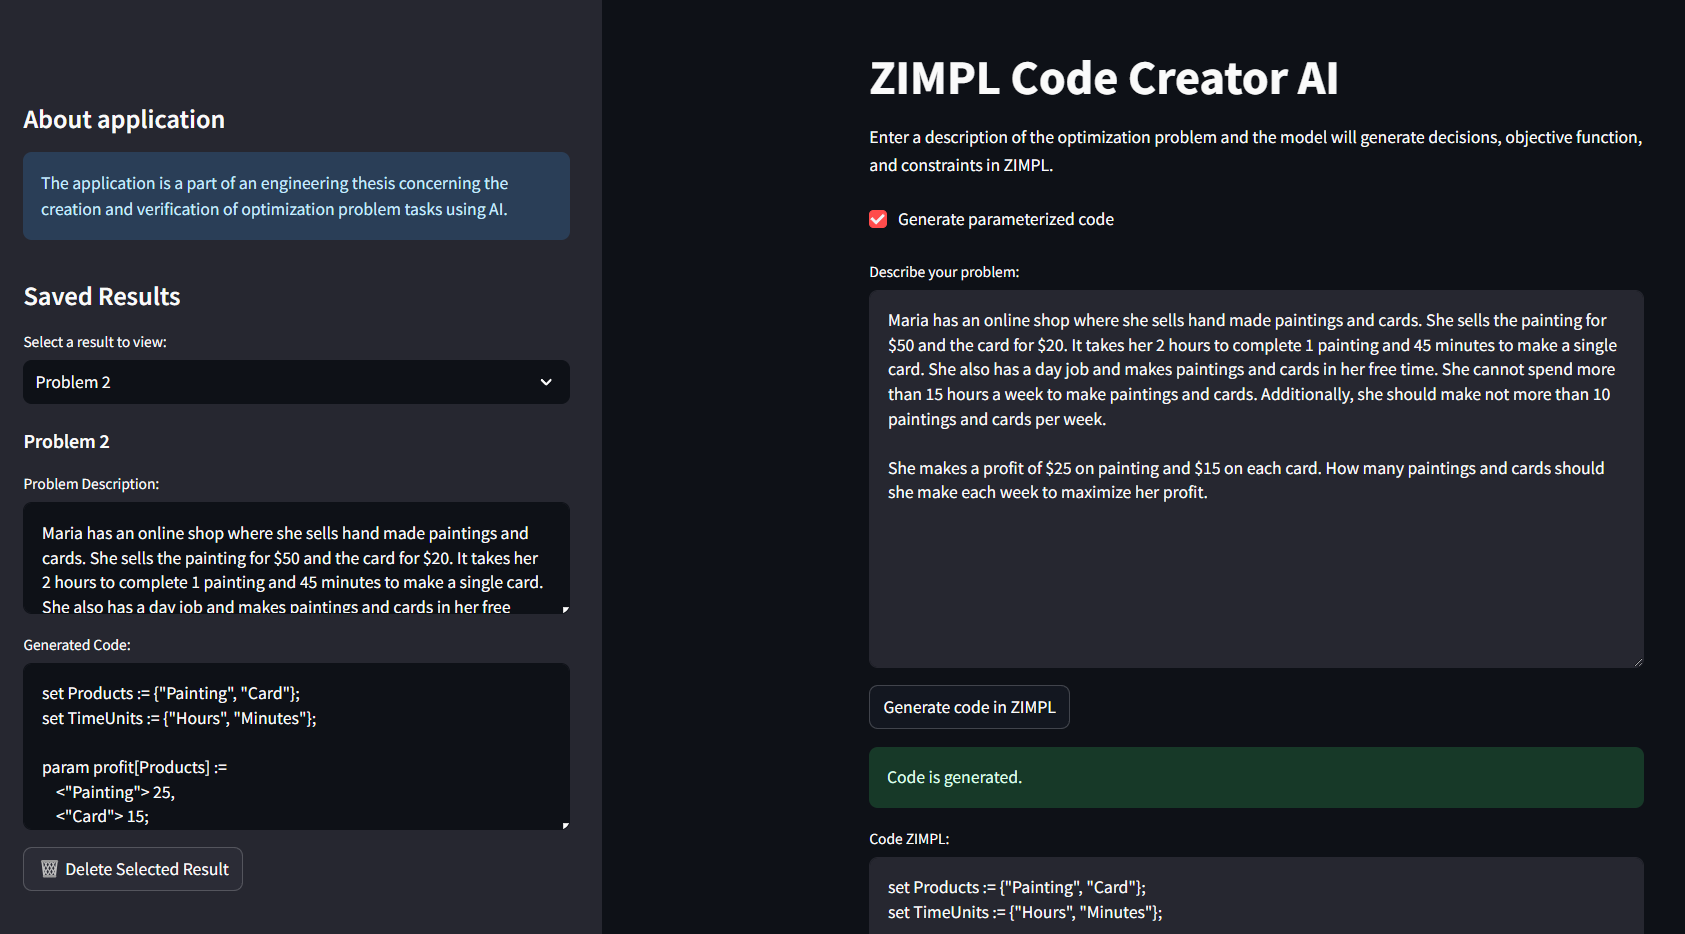
\includegraphics[width=1\linewidth]{figures/app.png}
    \caption{Wygląd interfejsu generatora kodu ZIMPL}
    \label{fig:gui}
\end{figure}

Na Rysunku \ref{fig:application-diagram} przedstawiono schemat graficzny ekranu generatora wraz z~układem jego funkcjonalności. Na Rysunku~\ref{fig:gui} znajduje się zrzut ekranu interfejsu użytkownika.